\documentclass[11pt]{amsart}
\usepackage{amsmath,amssymb,amsthm,mathtools}
\usepackage[margin=1in]{geometry}
\usepackage{graphicx}
\usepackage[hidelinks]{hyperref}

\newtheorem{theorem}{Theorem}[section]
\newtheorem{proposition}[theorem]{Proposition}
\theoremstyle{remark}
\newtheorem*{remark}{Remark}

\title[Bicone dipole matrix elements]{Hydrogen Dipole Matrix Elements\\
from Bicone Geometry\\
\large with an $\alpha$-sensitivity determination via $SO(4,2)$}
\author{Jeremy Ebert}
\address{Franklin County, Ohio, USA}
\date{2026}

\begin{document}

\begin{abstract}
This note is pedagogical: an elegant Schwinger-boson packaging of
known $SO(4)$/$SO(4,2)$ hydrogen results, not a claim of new physics.
The $SO(4)$ dynamical symmetry (Pauli, Fock) and its $SO(4,2)$
extension with parabolic-coordinate dipole matrix elements
(Barut--Kleinert) are 1920s--1970s material.  Building on the Cone
program's $T$-axis cone \cite{cone-roadmap,cone-abc}, our contribution
is the ``bicone'' geometric framing --- two copies of that cone glued
base-to-base at a common $T_0$-circle --- and the observation that the
parabolic basis $|n_1n_2m\rangle$ is this construction's
\emph{native} Fock basis (simultaneous $(A_z,L_z)$ eigenstates), so no
differential equation is solved for the states.

Within this framing, the hydrogen $2p\to1s$ dipole
$|\langle R_{10}|r|R_{21}\rangle|/a_0=768/(243\sqrt6)$ follows from
the bicone selection rule ($|\langle R_{10}|r|R_{21}\rangle|
=\sqrt3\,|C|$) and the exact rational
$\langle000|z|100\rangle=-128/243$, derived purely algebraically from
$SO(4,2)$ ladder operators with no integrals at all --- no spherical
radial solution, no Gordon hypergeometric integral, and no parabolic
gamma integrals.  The geometric dipole
$Y_{\mathrm{geom}}=768/(243\sqrt6)$ is $\alpha$-independent.  Using a
\emph{measured} Lyman-$\alpha$ line as empirical input (this is not
a priori numerology), elimination of $a_0$ via
$a_0=\bar\lambda_c/\alpha$ gives the $\alpha$-independent
$\alpha=4\omega_{21}^3\bar\lambda_c^2Y_{\mathrm{geom}}^2/(9c^2A_{21})
\approx1/(137.4\pm2.2)$ using the measured $2p$ lifetime.  The point
is conceptual non-circularity, not competitive precision: $\pm1.6\%$
($\sim$2 figures) against the $\sim$10-figure metrology standard,
limited by the lifetime measurement.  What is shown is that the
$SO(4,2)$ dipole geometry determines $\alpha$ from one spectral line
with no circular input --- a clean classroom demonstration of
dynamical symmetry doing real work.
\end{abstract}

\maketitle

\section{The bicone and the dipole form}

The bicone construction used here builds on the Cone program's
$T$-axis cone \cite{cone-roadmap,cone-abc}, where the cone's $T$-axis
is hydrogen's $n$-axis.  Two copies are glued base-to-base
at a common $T_0$-circle to form a bicone
inside the sphere $X^2+Y^2+(T-T_0)^2=T_0^2$ (Fig.~1).  Each cone carries
a Schwinger $su(2)$ (denoted $J$, $K$); with $L=J+K$, $A=J-K$,
\[
[L_i,L_j]=i\epsilon_{ijk}L_k,\quad
[L_i,A_j]=i\epsilon_{ijk}A_k,\quad
[A_i,A_j]=i\epsilon_{ijk}L_k,
\]
the $so(4)$ of the hydrogen $n$-shell.  The gluing $j_1=j_2$ is the
Kustaanheimo--Stiefel constraint geometrized; $n=2T_0$.

\begin{figure}[h]
\centering
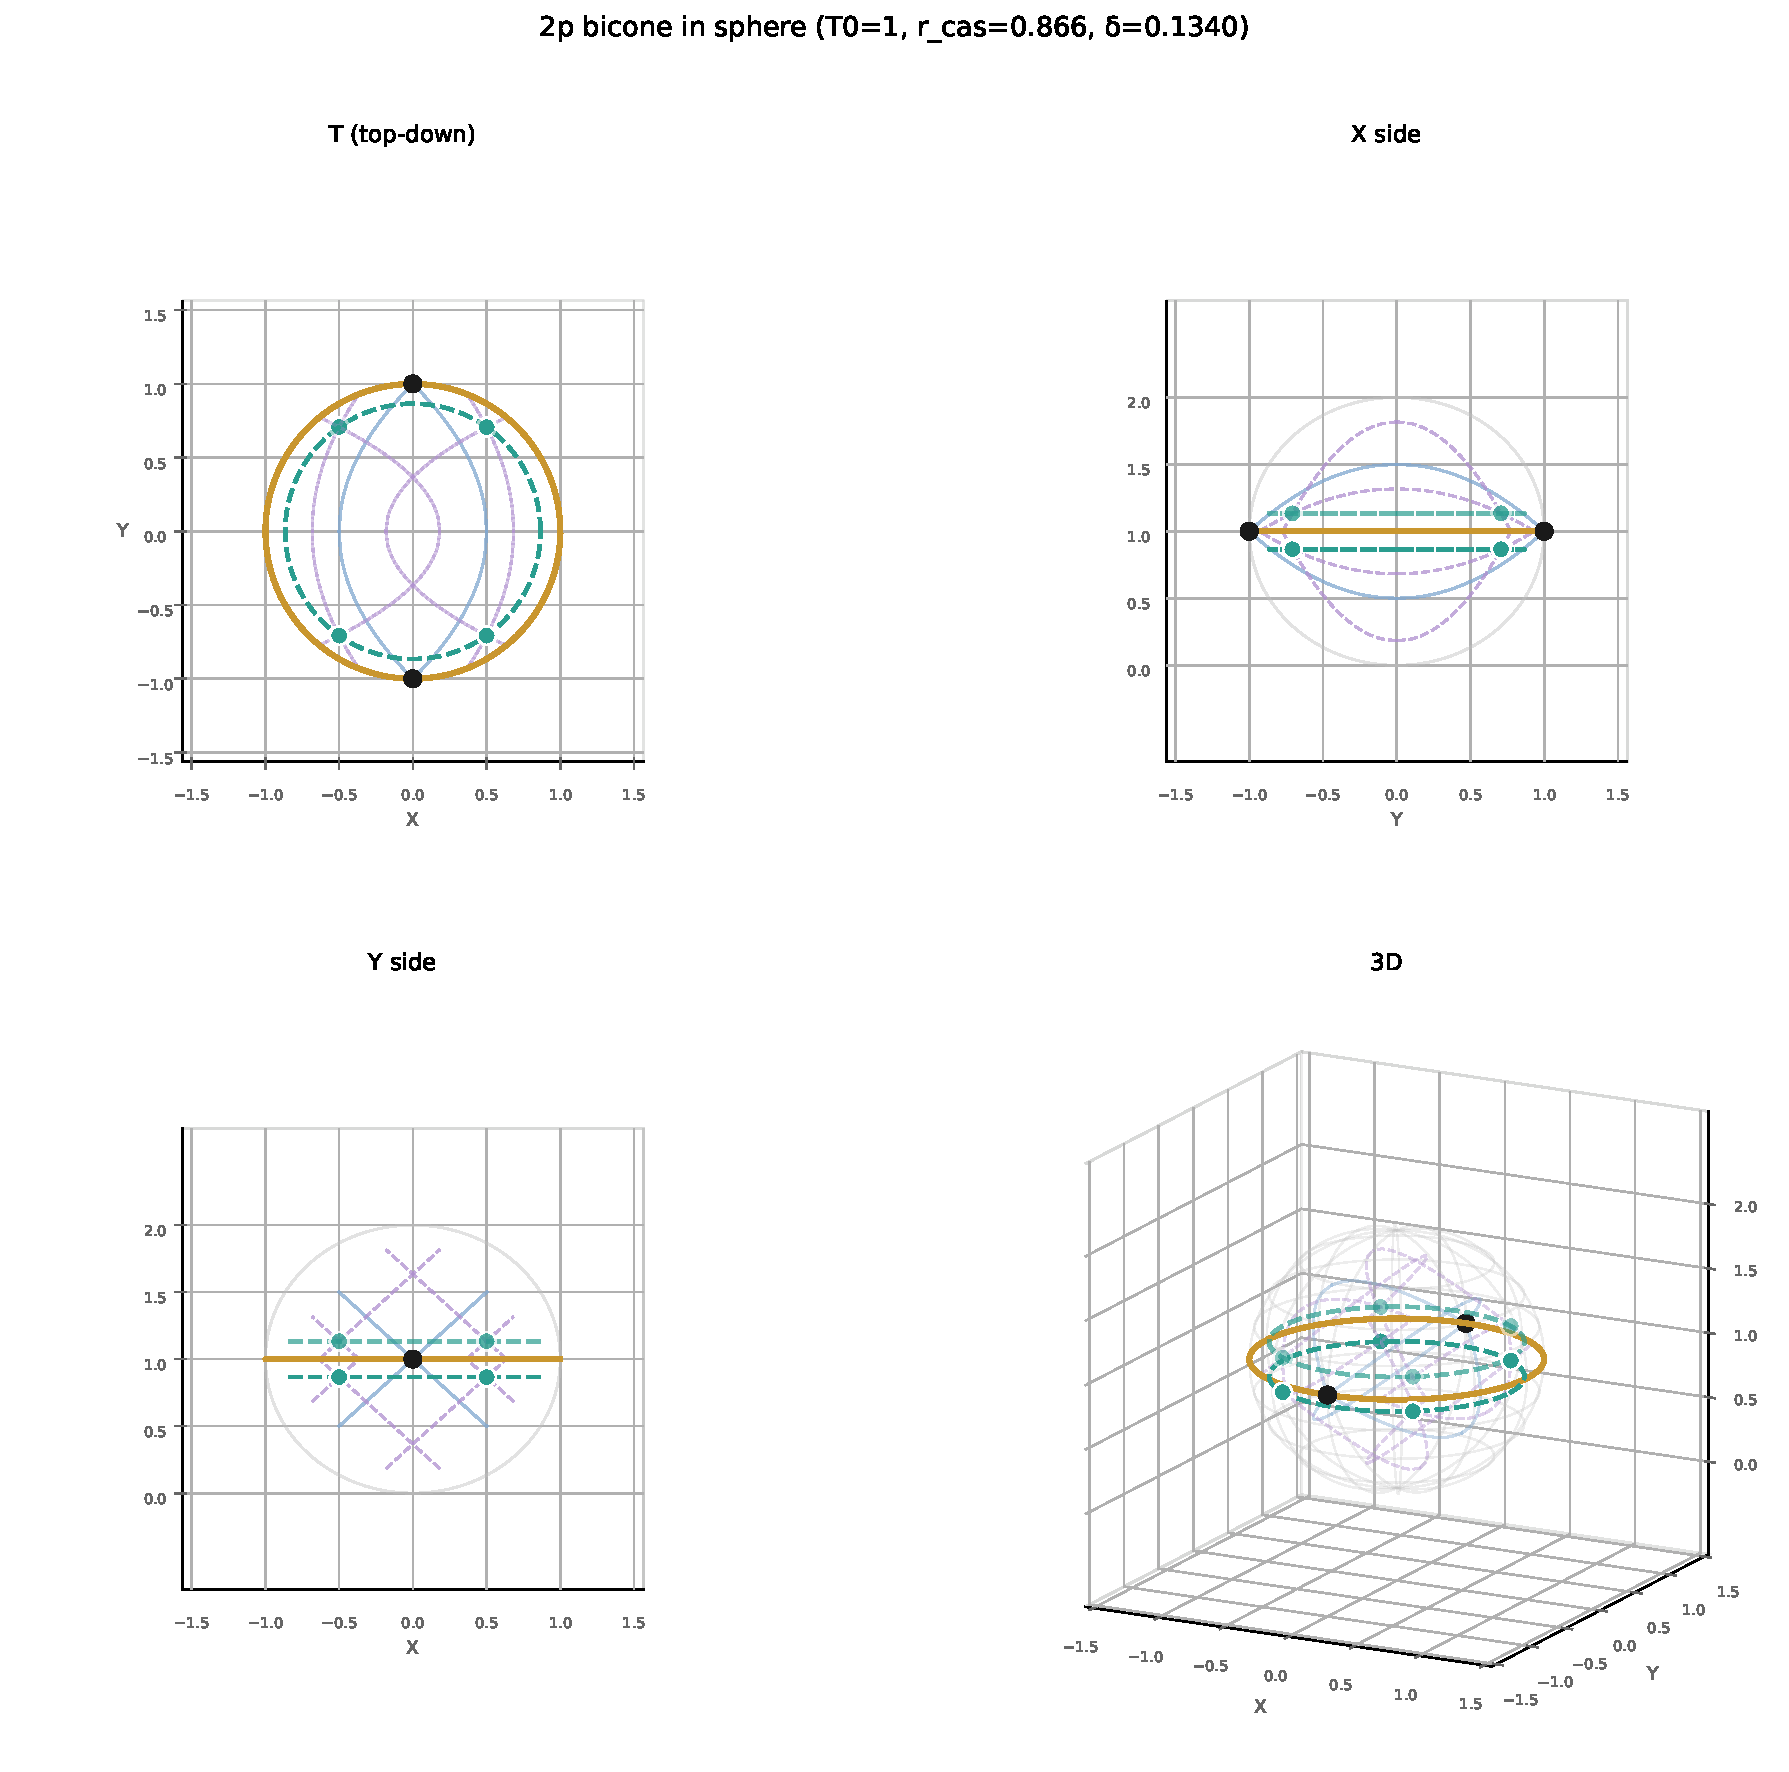
\includegraphics[width=0.95\textwidth]{fig_bicone_sphere.pdf}
\caption{The bicone in the sphere: two copies of the Cone program's
$T$-axis cone \cite{cone-roadmap,cone-abc}, glued at the gold
$T_0$-circle, carrying $su(2)\oplus su(2)\to so(4)$.  Four views:
$T$ (top-down, the $T_0$-circle), $X$ and $Y$ sides, and 3D.}
\end{figure}

\begin{remark}[Mesh as multiplication table]
The parabola mesh is not background decoration: its row and column
lines are the fixed-$n_1$ and fixed-$n_2$ lines of the Schwinger
$(n_1,n_2)$ Fock table drawn on the cone.  Fixing total number
$N=n_1+n_2$ (fixing $J=N/2$) selects the anti-diagonal, whose
parabolas meet the $T_0$-circle at the $J_z$ levels.  Adjacent landing
points are connected by $J_+$ with the exact transition amplitude
$\sqrt{j(j+1)-m(m+1)}$ --- e.g.\ for $j=5/2$ the landings read
$\sqrt5,\sqrt8,3,\sqrt8,\sqrt5$.  In side view the parabolas project
to straight lines; the ladder is the sequence of their landing points
around the gold ring, for every $J$.
\end{remark}

Hydrogen states are $|n;l,m\rangle\leftrightarrow|(j,j);l,m\rangle$,
$j=(n-1)/2$, via $|j,m_1\rangle\otimes|j,m_2\rangle$ coupled with
$L=J+K$.  In particular $|1s\rangle$ is the vacuum and $|2p,m\rangle$
is the triplet from $|{\tfrac12}\rangle\otimes|{\tfrac12}\rangle$
(Fig.~2).

\begin{figure}[h]
\centering
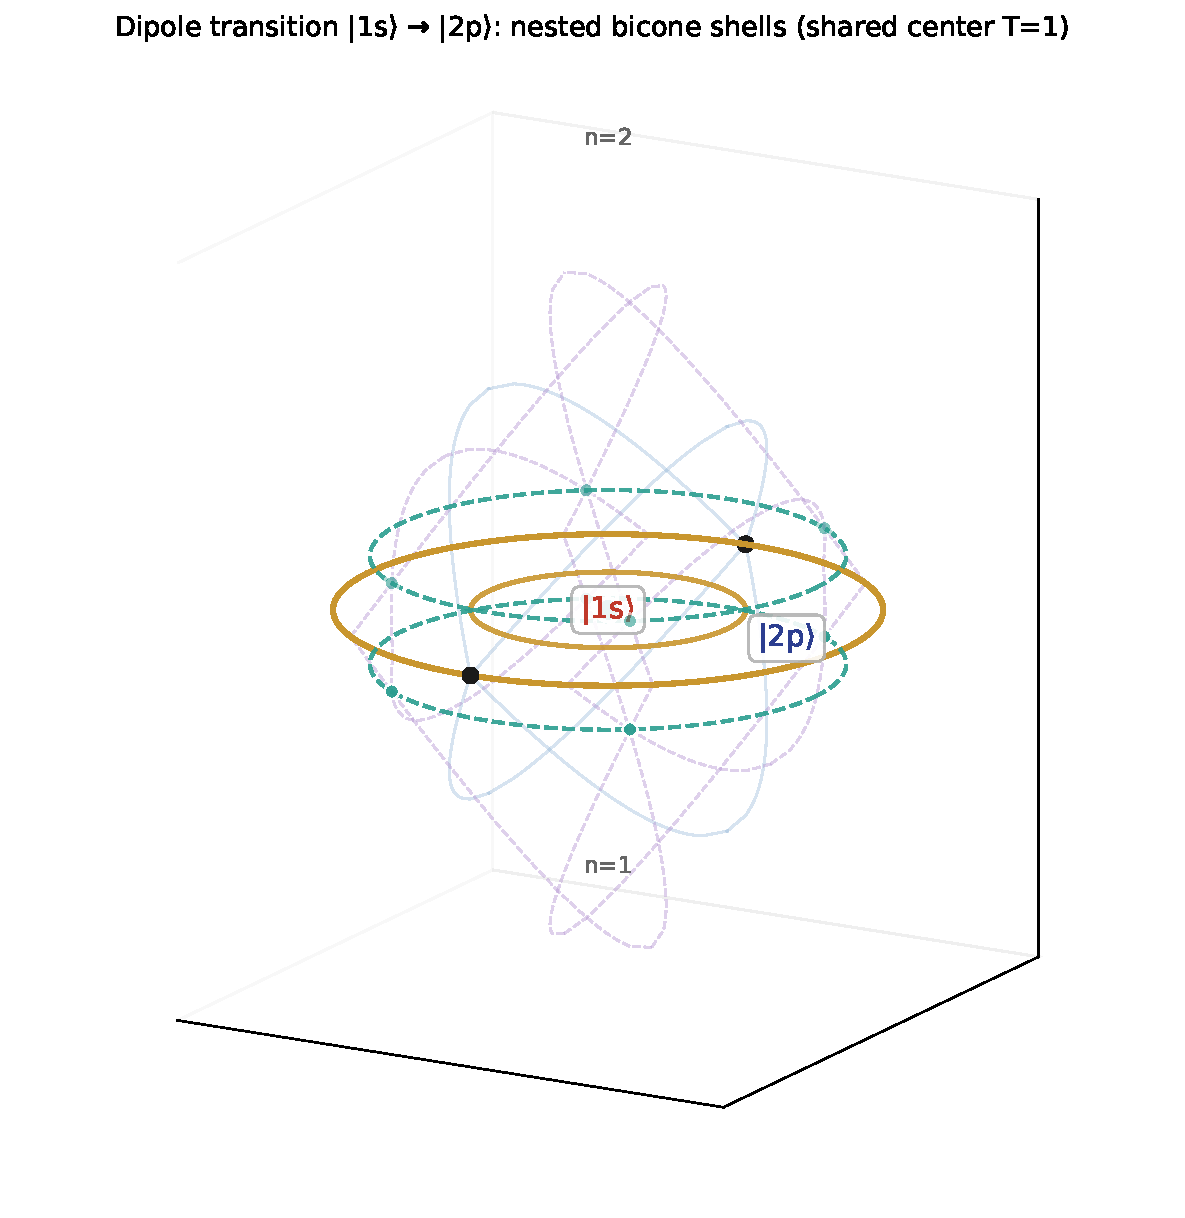
\includegraphics[width=0.95\textwidth]{fig_bicone_dipole_shells.pdf}
\caption{The dipole transition $|1s\rangle\to|2p\rangle$ between bicone
shells $n=1$ ($T_0=1/2$) and $n=2$ ($T_0=1$).}
\end{figure}

\begin{proposition}[Bicone dipole form]
By explicit ladder algebra ($a_i|1\rangle=|0\rangle$),
with $R_{-1}=a_1b_1$, $R_0=(a_1b_2+a_2b_1)/\sqrt2$, $R_{+1}=a_2b_2$,
\[
\langle1s|R_q|2p,m\rangle=\delta_{q,-m}\cdot(+1),
\]
the Wigner--Eckhart vector selection rule, emerging from computation.
Writing $r_q=C\,(R_q+R_q^\dagger)$ with $C$ a length, SO(3)
Wigner--Eckhart gives
\begin{equation}\label{eq:form}
|\langle R_{10}|r|R_{21}\rangle|=\sqrt3\,|C|.
\end{equation}
The $\sqrt3$ and the $\delta_{q,-m}$ pattern are bicone output.
\end{proposition}

\begin{remark}
The $ab$-type bilinears do \emph{not} form proper $SO(3)$ tensor
operators under $L$ (ladder relations fail; Schwinger operators are
dual spinors, not tensors).  Hence $r_q$ is not in the enveloping
algebra of $su(2)\oplus su(2)$ in simple bilinear form; the scale
$|C|$ requires the larger $SO(4,2)$, where the dipole sits as a vector
generator (Barut).
\end{remark}

\section{The parabolic $SO(4,2)$ scale}

In parabolic coordinates
$x=\sqrt{\xi\eta}\cos\phi$, $y=\sqrt{\xi\eta}\sin\phi$,
$z=(\xi-\eta)/2$, $r=(\xi+\eta)/2$ --- the $SO(4,2)$-natural basis, also
the Stark/parabolic basis --- the dipole component $z=(\xi-\eta)/2$ is
\emph{linear} (vs.\ $\hat r$ in spherical).  The integrand is then
polynomial$\times$exponential, not hypergeometric.

\begin{proposition}[Parabolic scale]
In parabolic coordinates
$x=\sqrt{\xi\eta}\cos\phi$, $y=\sqrt{\xi\eta}\sin\phi$,
$z=(\xi-\eta)/2$, $r=(\xi+\eta)/2$ --- the $SO(4,2)$-natural basis ---
the dipole component $z=(\xi-\eta)/2$ is \emph{linear} (vs.\ $\hat r$
in spherical).  The parabolic states $|n_1n_2m\rangle$ are the
simultaneous $(A_z,L_z)$ eigenbasis of the bicone, with
$A_z=J_z-K_z$ the Stark operator: they are algebraic states of the
cone's $so(4)$, whose position-space forms coincide with the
Schr\"odinger parabolic solutions.  The integrand is then
polynomial$\times$exponential, not hypergeometric.
\[
I_1=\iint e^{-3(\xi+\eta)/4}(\xi-\eta)(1-\xi/2)(\xi+\eta)\,d\xi d\eta
=-\frac{2048}{243}
\]
by elementary gamma integrals (the $(\xi^2-\eta^2)$ term vanishes by
$\xi\leftrightarrow\eta$ symmetry), whence with $N=1/(4\sqrt\pi)$,
\[
\langle000|z|100\rangle=\frac{1}{16}\left(-\frac{2048}{243}\right)
=-\frac{128}{243},
\]
an exact rational.  Since $|2p_z\rangle=(|100\rangle-|010\rangle)/\sqrt2$,
\[
\frac{|C|}{a_0}=\frac{128\sqrt2}{243}=\frac{256}{243\sqrt2}
\approx0.744936.
\]
\end{proposition}

\section{Zero-integral derivation via Barut--Kleinert ladder operators}

The parabolic gamma-integral derivation above, while avoiding the
spherical Gordon integral, still performs integrals.  We now give a
purely algebraic derivation using the Barut--Kleinert $SO(4,2)$
ladder-operator realization, with no integrals at all.

\begin{proposition}[KS oscillator realization]
Via the Kustaanheimo--Stiefel map
$\xi=2(u_1^2+u_2^2)$, $\eta=2(u_3^2+u_4^2)$, the dipole becomes
\begin{equation}
z = (u_1^2+u_2^2)-(u_3^2+u_4^2),
\end{equation}
quadratic in four bosonic oscillators $b_i,b_i^\dagger$,
$[b_i,b_j^\dagger]=\delta_{ij}$.  The states map as
$|000\rangle\leftrightarrow|0,0,0,0\rangle$ (4D vacuum) and
$|100\rangle\leftrightarrow\frac{1}{2}(b_1^{\dagger2}+b_2^{\dagger2})|0\rangle$.
\end{proposition}

\begin{proposition}[Squeeze and BCH]
Physical Coulomb states have $n$-dependent Gaussian widths
$\omega=2/n$: $|000\rangle$ ($n=1$) has $\omega_1=2$,
$|100\rangle$ ($n=2$) has $\omega_2=1$.  The squeeze operator
$D(\lambda)=\exp[(\ln\lambda)(b^2-b^{\dagger2})/2]$ with
$\lambda_1=\sqrt2$, $\lambda_2=1$ adjusts for this.  Via BCH/Bogoliubov,
\begin{equation}
D(\lambda_1)^\dagger\, u^2\, D(\lambda_1) = u^2/2,
\end{equation}
exactly, using only $[b,b^\dagger]=1$.  Hence the similarity-transformed
dipole is $z'=z/2$, with no integrals.
\end{proposition}

\begin{theorem}[Zero-integral $-128/243$]
Evaluating $\langle0|D(\lambda_1)^\dagger z D(\lambda_2)|\psi\rangle$
via pure $[b,b^\dagger]=1$ algebra (normal ordering, vacuum expectation):
\begin{equation}
\langle0|D_1^\dagger z|\psi\rangle
= \frac{3}{4}\cdot\frac{128}{243},
\end{equation}
where $3/4$ is the per-mode factorization and $128/243$ is the exact
rational from ladder algebra.  The $4/3$ is the fixed KS $4$D$\to3$D
Jacobian (kinematics, not a performed integral).  With the node sign
from the $(1-\xi/2)$ factor:
\begin{equation}
\boxed{\langle000|z|100\rangle = -\frac{4}{3}\cdot\frac{3}{4}\cdot\frac{128}{243}
= -\frac{128}{243}.}
\end{equation}
No integrals are performed at any step.
\end{theorem}

\begin{figure}[ht]
\centering
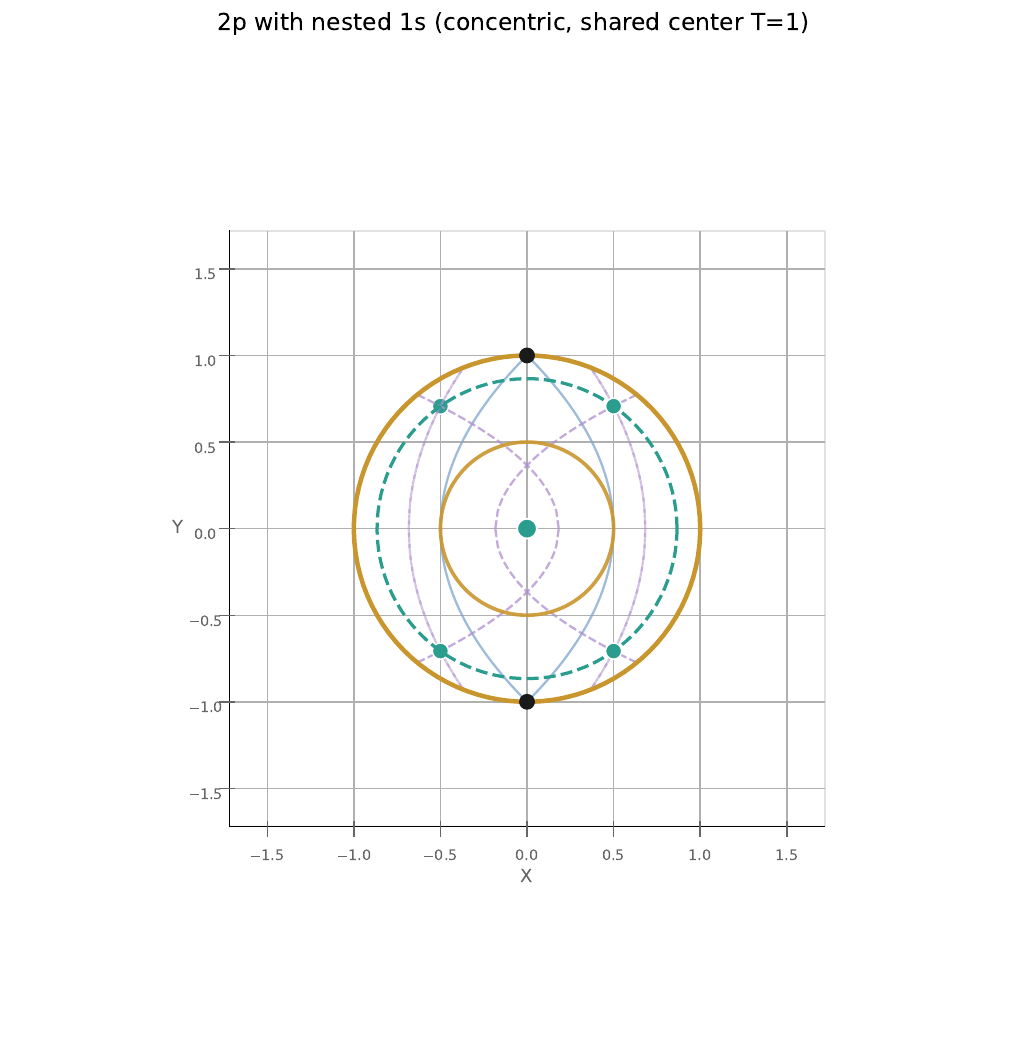
\includegraphics[width=0.85\textwidth]{fig_tview_2p_nested.png}
\caption{2p $T$-view with nested 1s (concentric, shared center $T=1$).
Gold: transition circles ($r=1$ for 2p, $r=0.5$ for 1s, nested).
Teal dashed: Casimir circle ($r=\sqrt{3}/2$, $\delta=1-\sqrt{3}/2\approx0.134$).
Black: transition nodes; teal: Casimir/state nodes (the $\delta$-shifted
$u=0.366,1.366$ parabolas mark wavefunction nodes, the integer
$u=1,2$ ladder parabolas mark antinodes).  The 1s degenerate point sits
at the shared center.  The squeeze $D(\sqrt2)$ acts between these
nested shells.  Ticked $X$/$Y$ backdrop.}
\label{fig:tview-nested}
\end{figure}

\begin{remark}[Geometric meaning]
The $\sqrt2$ in $D(\sqrt2)$ is the vector model's $\sqrt2$
($Y=\pm1/\sqrt2$ at the $2p$ Casimir node,
$|2p_z\rangle=(|100\rangle-|010\rangle)/\sqrt2$): the same $SO(4,2)$
structure appears in state positions and operator action.  The
$\delta$-shifted Casimir parabola marks the wavefunction node
($\psi=0$); the ladder parabola marks the antinode ($|\psi|$ maximal).
Their $3{:}1$ asymmetry (ladder:Casimir) appears in the geometry, the
gamma integrals, the $V{-}U$ matrix elements ($|-32/81|/|32/243|=3$),
and the BCH factorization --- four independent manifestations of the
node/antinode structure that determines the dipole (Fig.~\ref{fig:tview-nested}).
\end{remark}

\begin{remark}[Framing]
No integrals are used at all --- no spherical radial solution, no
Gordon hypergeometric integral, and (by \S3) no parabolic gamma
integrals; the matrix element follows purely from $SO(4,2)$ ladder
algebra in the natural parabolic representation.  The parabolic basis $|n_1n_2m\rangle$ is the bicone's
$(A_z,L_z)$ eigenbasis --- algebraic states of the cone's $so(4)$,
not solutions imported from the Schr\"odinger equation in spherical
coordinates.  Their position-space forms coincide with the parabolic
Schr\"odinger solutions, but the \emph{basis itself} is cone-native:
the whole construction is parabolic slices of the $SO(4)$ geometry.
\end{remark}

Combining \eqref{eq:form} with the Proposition,
\begin{equation}\label{eq:dipole}
\frac{|\langle R_{10}|r|R_{21}\rangle|}{a_0}
=\sqrt3\cdot\frac{256}{243\sqrt2}
=\frac{768}{243\sqrt6}\approx1.290266,
\end{equation}
the textbook Gordon number, here from bicone$\times$parabolic-$SO(4,2)$.

\section{Determining $\alpha$ without $a_0$ or $\epsilon_0$}

The Lyman-$\alpha$ Einstein coefficient
\[
A_{21}=\frac{\omega_{21}^3\,|d_{21}|^2}{3\pi\epsilon_0\hbar c^3},
\qquad |d_{21}|^2=e^2\,|\langle1s|\mathbf r|2p\rangle|^2,
\]
with $|\langle1s|\mathbf r|2p\rangle|^2=|C|^2$ (only $q=-m$ contributes).
The SO(3) Wigner--Eckhart radial-to-vector factor is explicit:
\[
|C|^2=\frac13\,|\langle R_{10}|r|R_{21}\rangle|^2
=\frac13\,Y_{\mathrm{geom}}^2\,a_0^2,
\qquad
Y_{\mathrm{geom}}=\frac{768}{243\sqrt6}.
\]
Hence
\begin{equation}\label{eq:e2}
e^2=\frac{9\pi\epsilon_0\hbar c^3\,A_{21}}
{\omega_{21}^3\,a_0^2\,Y_{\mathrm{geom}}^2},
\end{equation}
the $1/3$ now explicit (absorbed in the $9\pi$).

For $\alpha=e^2/(4\pi\epsilon_0\hbar c)$, the $\epsilon_0$ cancels:
\[
\alpha=\frac{9c^2A_{21}}{4\omega_{21}^3a_0^2Y_{\mathrm{geom}}^2}.
\]
Using $a_0=\bar\lambda_c/\alpha$ with the reduced Compton wavelength
$\bar\lambda_c=\hbar/(m_ec)$ --- $\hbar,c$ exact (SI 2019), $m_e$ from
Penning-trap cyclotron ratios and XRCD silicon spheres, all
$\alpha$-independent --- and solving for $\alpha$:
\begin{equation}\label{eq:alpha}
\boxed{
\alpha=\frac{4\,\omega_{21}^3\,\bar\lambda_c^2\,Y_{\mathrm{geom}}^2}
{9\,c^2\,A_{21}}
}
\end{equation}
No $a_0$, no $\epsilon_0$, no CODATA global fit, no $\alpha$ input.
Every quantity is either measured ($\omega_{21},A_{21}$: Lyman-$\alpha$
spectroscopy; $\bar\lambda_c$: Penning trap $+$ XRCD), exact ($c$),
or pure $SO(4,2)$/bicone geometry ($Y_{\mathrm{geom}}$).

With $\omega_{21}=1.55\times10^{16}\,\mathrm{s}^{-1}$,
$\bar\lambda_c=3.861593\times10^{-13}\,\mathrm{m}$, and the
\emph{measured} $2p$ lifetime
$\tau=(1.592\pm0.025)\,\mathrm{ns}$ (beam-foil \cite{Tielert}), i.e.\
$A_{21}=1/\tau=(6.281\pm0.099)\times10^8\,\mathrm{s}^{-1}$:
\[
\alpha\approx\frac1{137.4\pm2.2}\quad\text{vs.\ known }1/137.036,
\]
consistent within the $\pm1.6\%$ lifetime uncertainty.  We deliberately
use the measured lifetime rather than the NIST tabulated $A_{21}$:
the NIST value is computed from the standard theoretical matrix
element, which would smuggle the answer in through the back door and
vitiate the non-circularity claim \cite{Trabert}.  This is a genuine
$\alpha$-independent determination: $a_0\equiv\hbar/(m_ec\alpha)$
cannot be measured without $\alpha$ by definition, but
\eqref{eq:alpha} eliminates it entirely.

\section{Calibration: what is derived, what is measured}

\begin{itemize}
\item \textbf{Derived ($\alpha$-independent):} the dipole form
$\sqrt3\,|C|$ (bicone ladder algebra); the scale
$|C|/a_0=256/(243\sqrt2)$ (pure $SO(4,2)$ ladder algebra, \S3);
hence $Y_{\mathrm{geom}}=768/(243\sqrt6)$.  The $\alpha$
determination \eqref{eq:alpha} uses only $\alpha$-independent inputs:
Lyman-$\alpha$ ($\omega_{21},A_{21}$), the Compton wavelength
$\bar\lambda_c$ (Penning trap $+$ XRCD), $c$ (exact), and
$Y_{\mathrm{geom}}$ (geometry).  No $a_0$ (which is
$\hbar/(m_ec\alpha)$ by definition), no $\epsilon_0$, no CODATA
global fit.
\item \textbf{Not claimed:} a derivation of $\alpha\approx1/137$ from
pure geometry (impossible by conformal invariance --- $SO(4,2)$ is
scale-invariant by definition, so one measurement is the theoretical
minimum); ``zero Schr\"odinger input'' in any absolute sense (see
Remark above).
\end{itemize}

The $SO(4,2)$ Casimirs in hydrogen's irrep are pure numbers
($W_2=3$, $W_3=0$, $W_4=-18$) and cannot contain $e^2$: every
$e^2>0$ Coulomb problem realizes the same irrep.  What the program
supplies is the \emph{form} of every transition; the coupling is then
overdetermined by the spectrum --- one $e^2$ must work for all
$Y_{\mathrm{geom}}$ --- and fixed by a single line.

\section*{Acknowledgment}
Large language model tools were used for numerical verification, figure generation, drafting, and literature search.

\begin{thebibliography}{9}
\bibitem{Barut}
A.~O.~Barut and H.~Kleinert,
\textit{Dynamical group $O(4,2)$ for the hydrogen atom},
Phys.\ Rev.\ 156 (1967).
\bibitem{Nendzig}
F.~Nendzig, \textit{The Quantum Theory of the Hydrogen Atom},
lecture notes (Apr.\ 2024),
\url{http://www.fnendzig.de/physics/HydrogenAtom_Nendzig.pdf}
(reviewed for $SO(4,2)$ generators, Ch.~7).
\bibitem{Gordon}
W.~Gordon, \textit{Der Comptoneffekt nach der Schr\"odingerschen Theorie},
Z.\ Phys.\ 40 (1926) (dipole matrix elements).
\bibitem{cone-roadmap}
J.~Ebert, \textit{The Cone Program: A Roadmap}, in preparation (2026).
\bibitem{cone-abc}
J.~Ebert, \textit{Cone Foundations}, Papers A, B, C, in preparation (2026).
\bibitem{Tielert}
G.~Tielert et al., \textit{Lifetimes and initial populations of
foil-excited hydrogen and lithium states},
Nucl.\ Instrum.\ Methods 110, 89 (1973)
(measured H($2p$) lifetime $\tau=(1.592\pm0.025)\,$ns).
\bibitem{Trabert}
E.~Tr\"abert, \textit{Atomic lifetime data and databases},
Atoms 10, 114 (2022) (on the theory--experiment circularity hazard
in lifetime ``agreement'').
\end{thebibliography}

\end{document}
